\documentclass[font=12pt]{paper}
\usepackage{gary}
\usepackage{subfigure}
\usepackage[margin=1in]{geometry}
\usepackage{mwe}
\title{Modeling Frequency of Terrorist Attacks}
\author{Gary Cheng and Preetham Gujjula}

\begin{document}
\maketitle 

\section{Introduction}
Global terrorism is a major issue today, and has been in the American zeitgeist at least since 9/11. Identifying patterns in attacks, and being able to predict future attacks, would be useful to law enforcement and the public. As absic studye decided on a dataset of terrorist attacks around the globe from 1970 to 2016. Studying this dataset allowed us to analyze how patterns of terrorist attacks have changed over time.

The dataset comes from the Global Terrorism Database, compiled by the National Consortium for the Study of Terrorism and Responses to Terrorism (START), located at the University of Maryland, College Park. From 1970 to 1997, the data was collected by the Pinkerton Global Intelligence Service (PGIS). “electronic news archives, existing data sets, secondary source materials such as books and journals, and legal documents”. 


\section{Data Analysis}
\subsection{Cleaning}
Our dataset contains every terrorist attack from 1970 to 2016. To form a time series out of this dataset, we counted the number of attacks that occurred each month. Figure ___ displays a plot of the number of attacks per month since 1970.

[PLOT HERE]

The data from 1998 to 2007 was collected retrospectively, as opposed to the other data, which was collected in real time. According to START, retrospective collection may underestimate the true number of terrorist attacks, because some media sources that documented the attacks are no longer available. Indeed, there is a subtle drop in the number of attacks in [plot above] for those years. Unfortunately, the magnitude of the undercounting is impossible to estimate, so we do not attempt to correct it.

Furthermore, the GTD defines a terrorist attack as “the threatened or actual use of illegal force and violence by a non-state actor to attain a political, economic, religious, or social goal through fear, coercion, or intimidation”. This is quite a broad definition, which is understandable, since the GTD aims to be as inclusive as possible, and allow researchers to filter the data according to their own criteria.

For these reasons (the variance in data collection methods over the years, and the broad definition of terrorist attack), we filtered the original dataset to select attacks that resulted in 10 casualties. Our rationale is that the likelihood of undercounting terrorist attacks of that magnitude is far less. Furthermore, attacks of this scale are more in line with what a layman would consider a terrorist attack. The plot of the filtered time series is rendered in figure __.

[PLOT HERE]

%\subsection{Interpolation}

There is a gap of 12 missing data points corresponding to the year 1993 because the data, which was collected by the Pinkerton Global Intelligence Service (PGIS), was lost before being transferred to START. To correct for this gap, we impute the data using the tsimpute library in R. Selecting an imputation method is difficult because it generally requires a model of the data first. Thus, we opted to use the simplest imputation method, which patches the missing data with a linear fit. Figure __ displays the time series with the imputed data.

[PLOT HERE]


%\subsection{Outliers}

Now we filter outliers from the dataset. The library tsoutliers provides a convenient way to identify different kinds of outliers in the dataset. We decided to only filter for additive offset, transient change, and innovational outliers, i.e., outliers manifested as spikes in the underlying dataset. We decided not to filter for level-shift outliers, since we expect to see level-shifts in the timeseries. We also didn’t filter for seasonal additive outliers, since we would not be surprised to see seasonal spikes or dips in the time series.

%\subsection{Final raw Time Series}
After filtering for 10 casualties, imputing the data, and removing outliers, the time series that we will be working with looks like this:

[PLOT HERE]

\subsection{Chasing Stationarity}
Visually, the original timeseries does not seem stationary. In particular, the mean of the series appears to increase as time progresses. In addition, the ACF of the timeseries, plotted in figure ___, decays slowly as the lag increases -- another indication that the series is not stationary.

[FIGURE HERE]

%\subsection{Logged Data}

One potential method to derive a stationary timeseries is to take the log of the data in the original series. This method would be highly suitable if the original series has an exponentially growing trend. The growth in our original series looks vaguely exponential, which justifies trying to log-transform the series.

However, in our case, this method is problematic, since the original series has 0 values, and log 0 is undefined. We could replace the 0 values with some small positive epsilon value, as a potential fix. Unfortunately, log(x) -> -infinity as x -> 0+, so taking log(epsilon) would result in an extremely negative value. This value would also depend a lot on our choice of epsilon, and there is no straightforward way to choose an epsilon. For this reason, we opted not to log-transform the data.

%\subsection{Diffed Data}
In lieu of using a log-transform, we tried differencing and twice-differencing the dataset as a method of obtaining a stationary dataset. The ACFs of these datasets are plotted in figure ___.

[FIGURES HERE]

The sharp drop-off in the ACFs of these datasets suggests that they are both stationary.

For a more quantitative measure of stationarity, we used the augmented Dickey-Fuller test on these two time series. The differenced series had a DF_t statistic of ___ and the twice-differenced series had a DF_t statistic of ___. These results correspond to p-values of ___ and ___ respectively, meaning that at the __% significance level, we reject the null-hypotheses of unit roots in either of these time series, and accept the alternative hypotheses that these series are stationary.


\subsection{Model Selection}
%EACF

To obtain a set of potential ARIMA models that fit our time series, we use the extended sample autocorrelation function (ESACF) method. In this method, we generate a table of sample ACFs for ARMA(p, q) models, where p and q lie in a small range, and use this table to select promising models for further analysis.

The ESACF tables (generated by the eacf function in R) for the differenced and twice-differenced time series are shown below. A 0 in a table-entry indicates a non-significant ACF, and an x indicates a significant ACF. We are interested in models with non-significant ACFs because ___.

[FIGURES HERE]

From these tables, we selected the models ___ for further analysis. 

%Periodogram for seasonality

The periodogram for the differenced data is shown below. For a more useful visual, we plot the smoothed periodogram below. Recall that in the smoothed periodogram, each value is replaced with the average of the L = 2m + 1 values around it. After experimenting around with our choice of m, we chose m = sqrt(n) with a split cosine bell with a taper of 0.1. These values gave us a reasonable looking periodogram that we could interpret.


%[FIGURE HERE]

In our smoothed and tapered periodogram, we see a peak around omega = 0.27, suggesting a seasonality in the data of $1/0.27 \approx 4$.

%AIC, BIC, MSE

To evaluate how well our models fit the data, we compute the AIC, BIC, and AICc for each of our 8 candidate models, in the table below.

From this table, we see that model ___ has low AIC, BIC, and AICC values, which makes it a promising candidate.

We also held out __ months of data, from 20-- to 20--, to validate each of our models. The mean squared error of each model’s forecast for the training data is displayed in the figure below.

[FIGURE HERE]

The ___ model has the lowest error on the training data. 

\subsection{Forecasting}

Based on our validation methods, we chose as ____ our final model. It has low AIC, BIC, and AICC values, and the prediction generated by this model for the years 20__ to 20__ has lowest mean squared error.

Using our final model, we generated a forecast of __ months, displayed in the figure below. The prediction fits the behavior of the data fairly well.






\begin{figure}
\centering
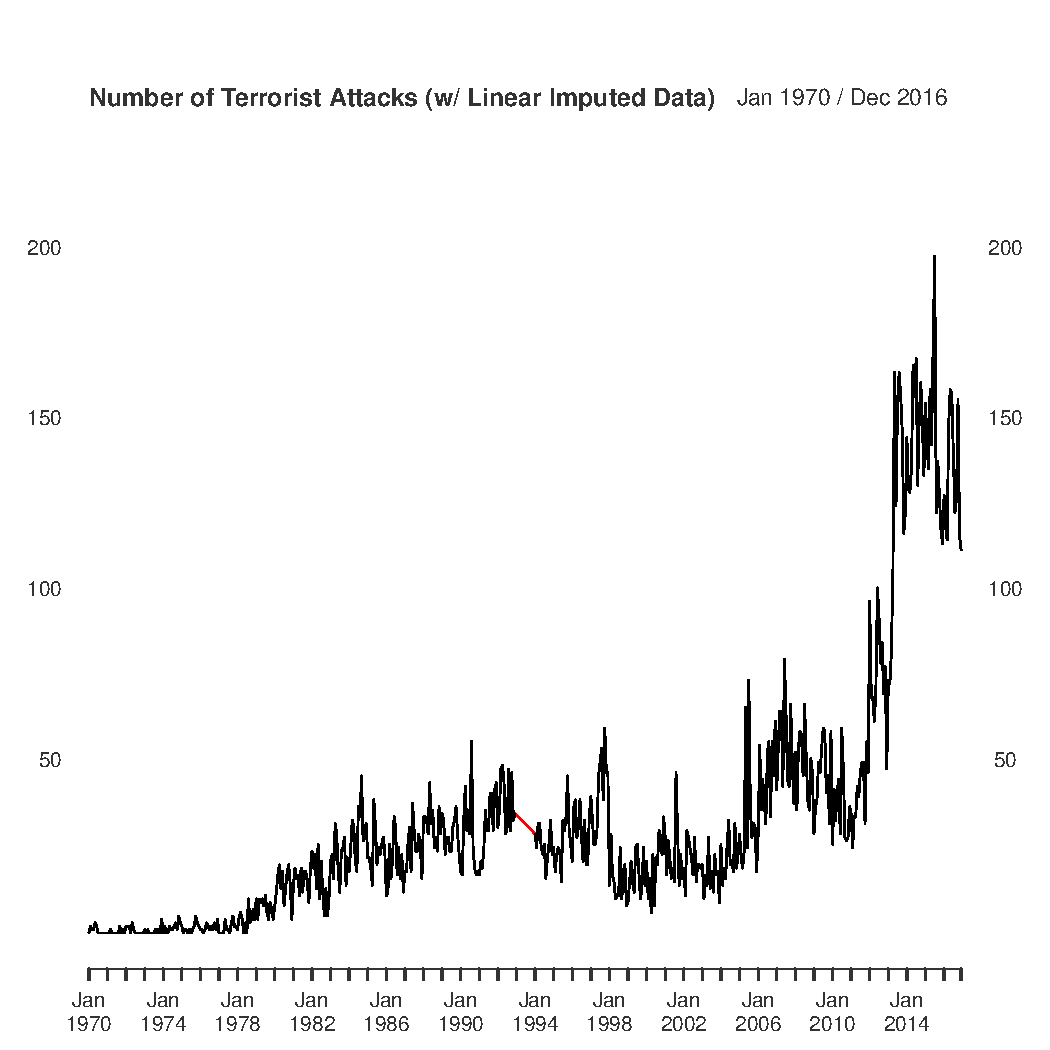
\includegraphics[width=0.75\linewidth]{../image/og_ts.pdf}
\caption{The original time series with a linear imputation (in red) for the missing data in 1993.}
\label{og}
\end{figure}

\begin{figure}
\centering
    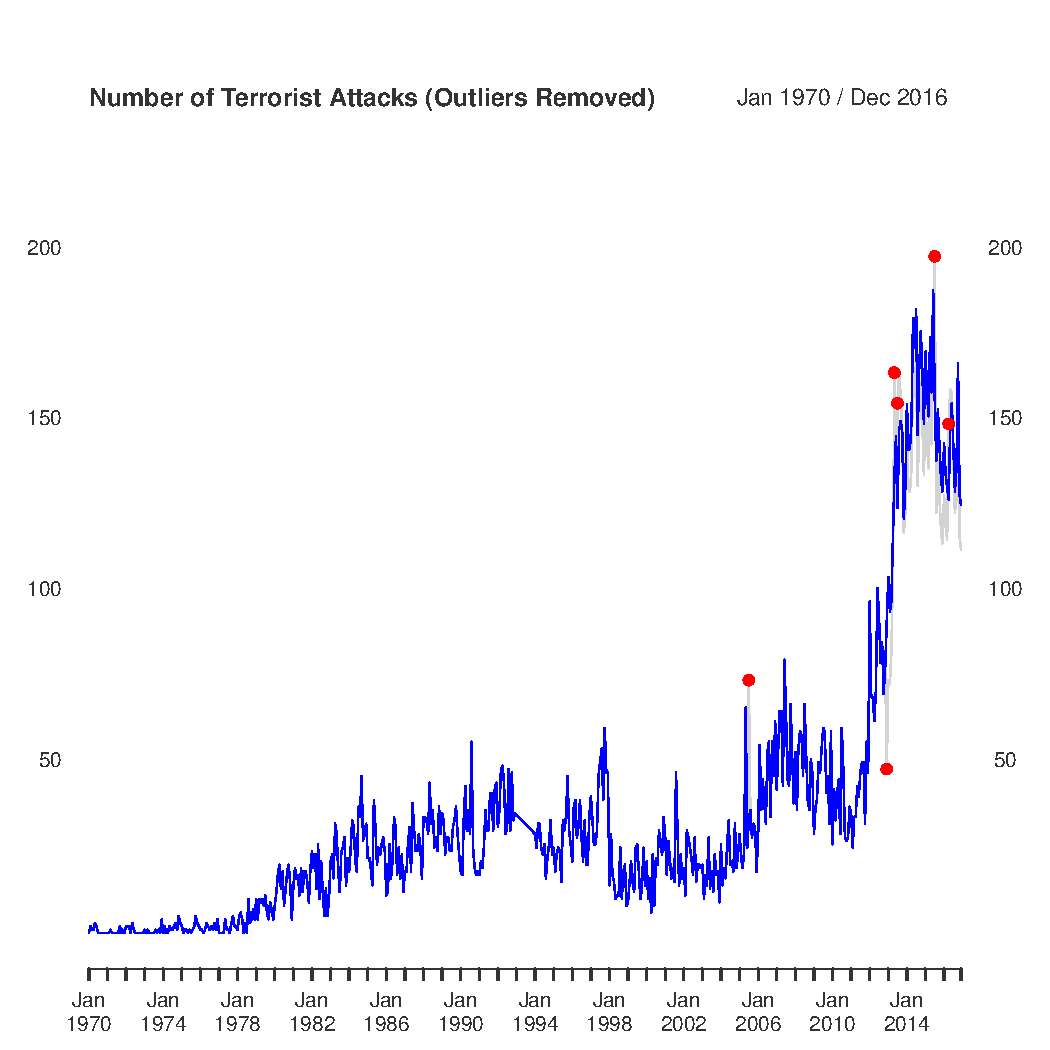
\includegraphics[width=0.75\textwidth]{../image/outlier_comparison.pdf}
\caption{The imputed time series (in blue) with outliers removed. The original time series shown in gray. The 6 outliers are shown in red. }
\label{outlier}
\end{figure}

\begin{figure}
\centering
    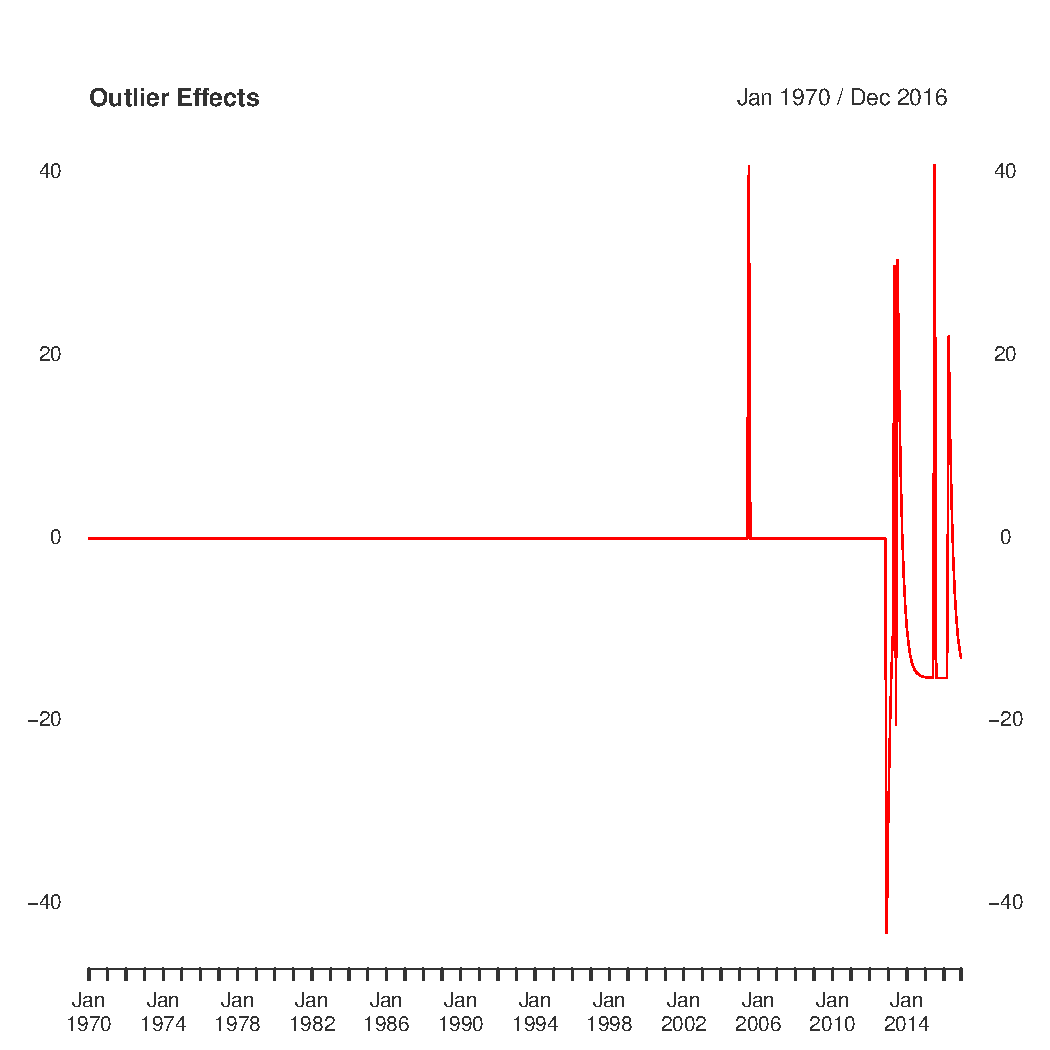
\includegraphics[width=0.75\textwidth]{../image/outlier_effects.pdf}
\caption{The outlier effects of the identitifed outliers are displayed here.}
\label{outlier}
\end{figure}



\begin{figure}
\centering
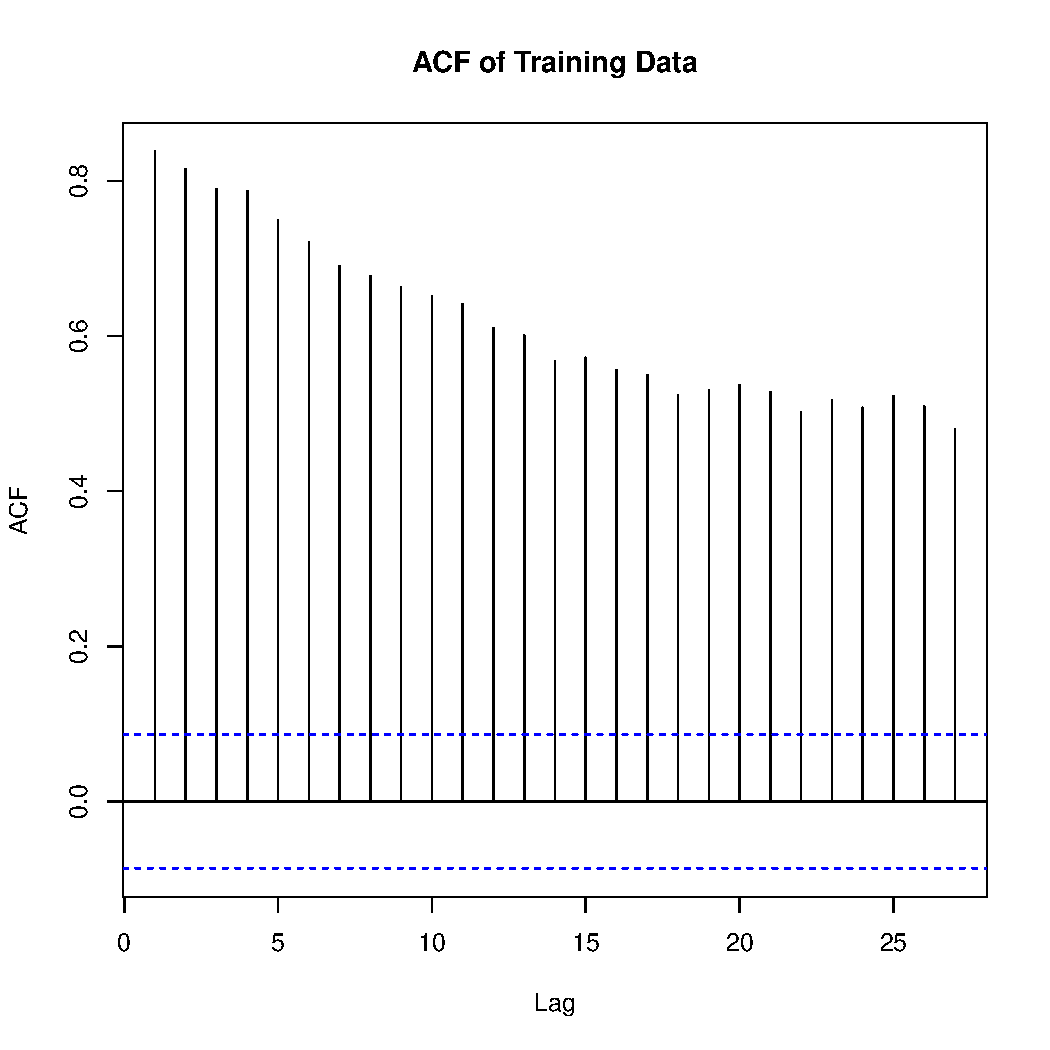
\includegraphics[width=0.45\linewidth]{../image/acf_og.pdf}
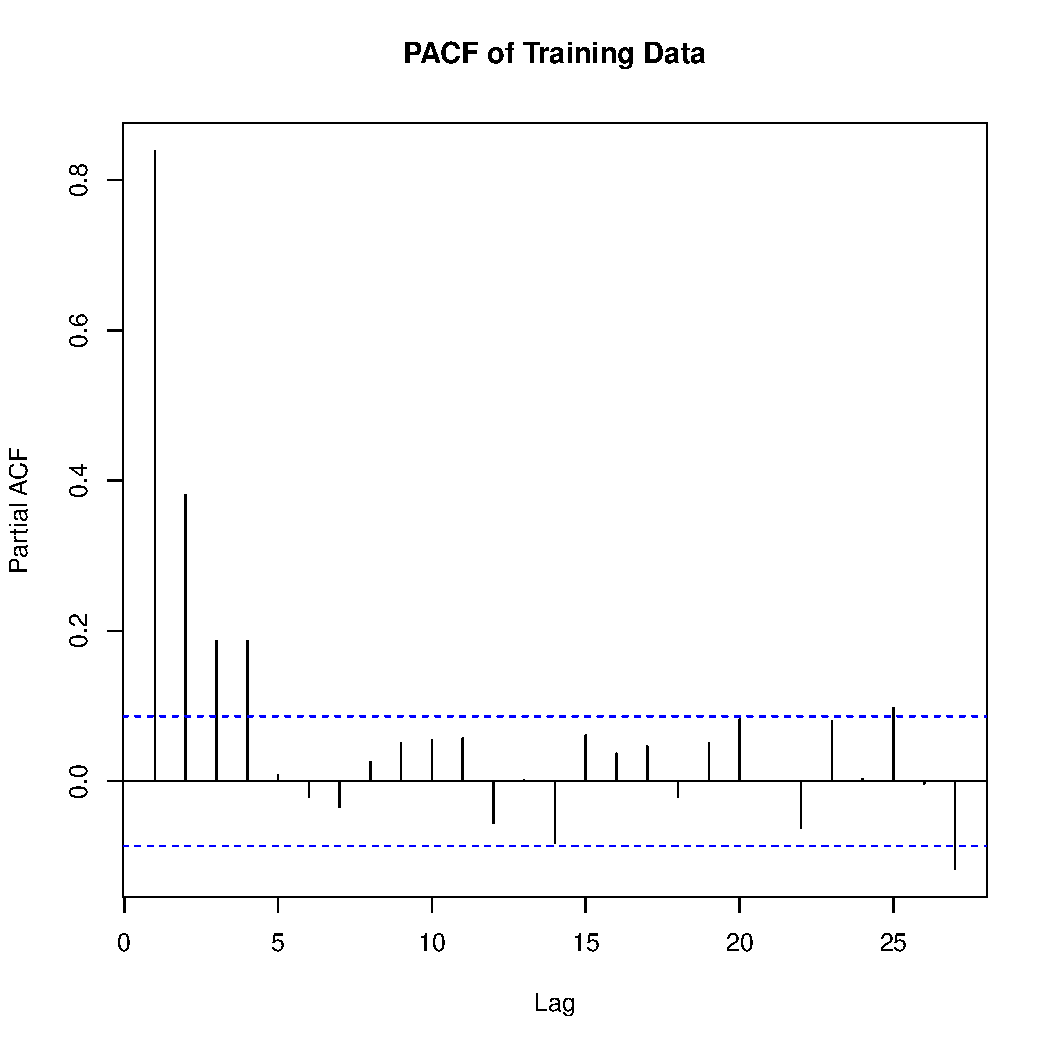
\includegraphics[width=0.45\linewidth]{../image/pacf_og.pdf}
\caption{The ACF and PACF of the time series}
\label{og_acf_pacf}
\end{figure}



\begin{figure}
\centering
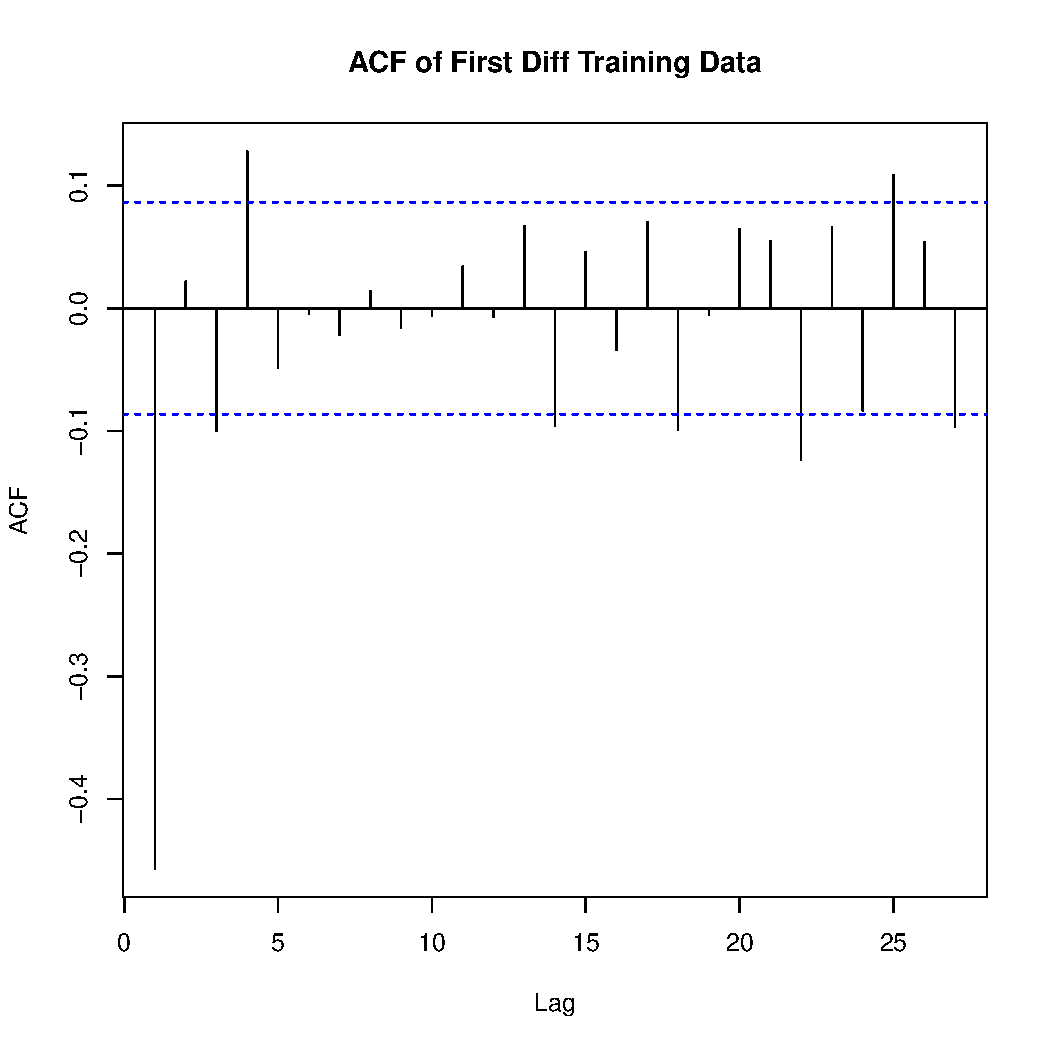
\includegraphics[width=0.45\linewidth]{../image/acf_first_diff.pdf}
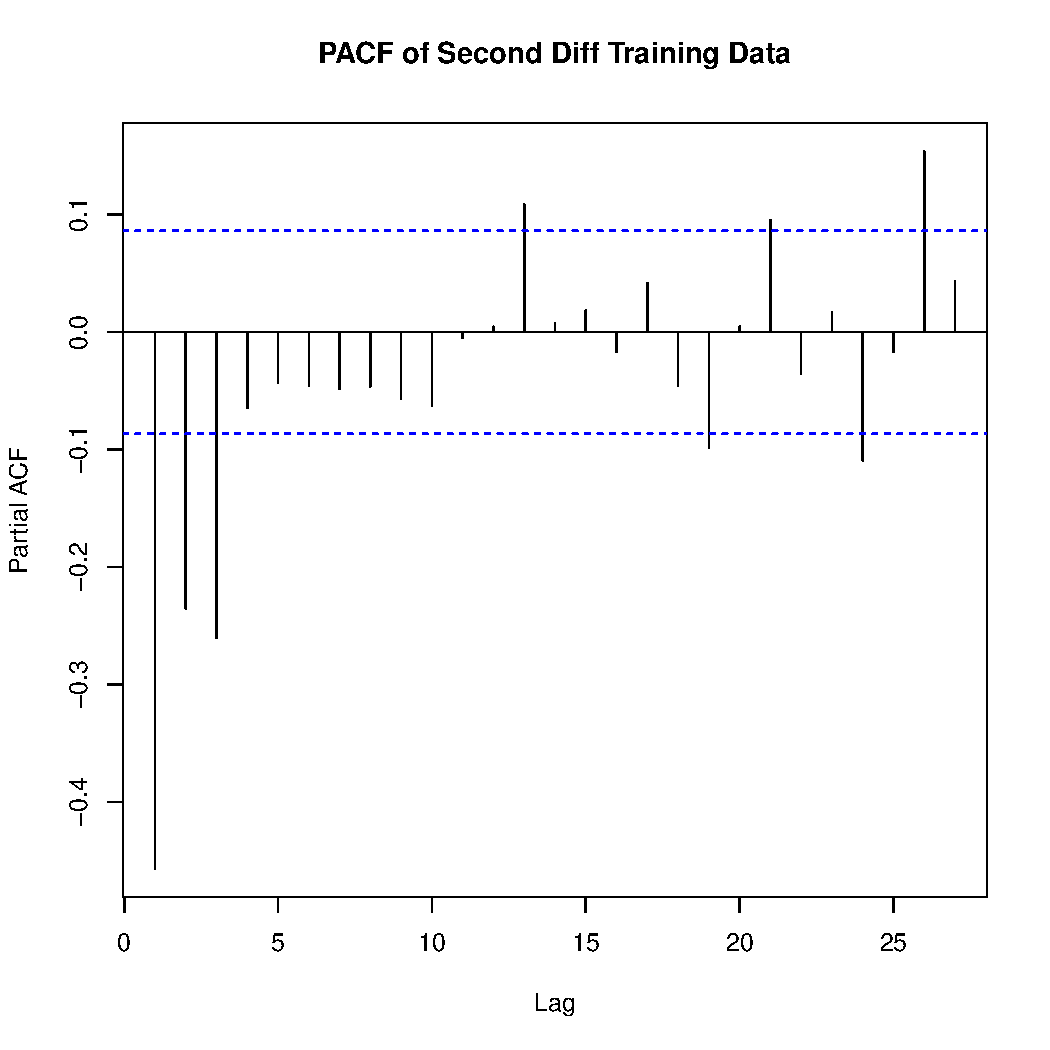
\includegraphics[width=0.45\linewidth]{../image/pacf_second_diff.pdf}
\caption{The ACF and PACF of the first diff time series}
\label{first_acf_pacf}
\end{figure}

\begin{figure}
\centering
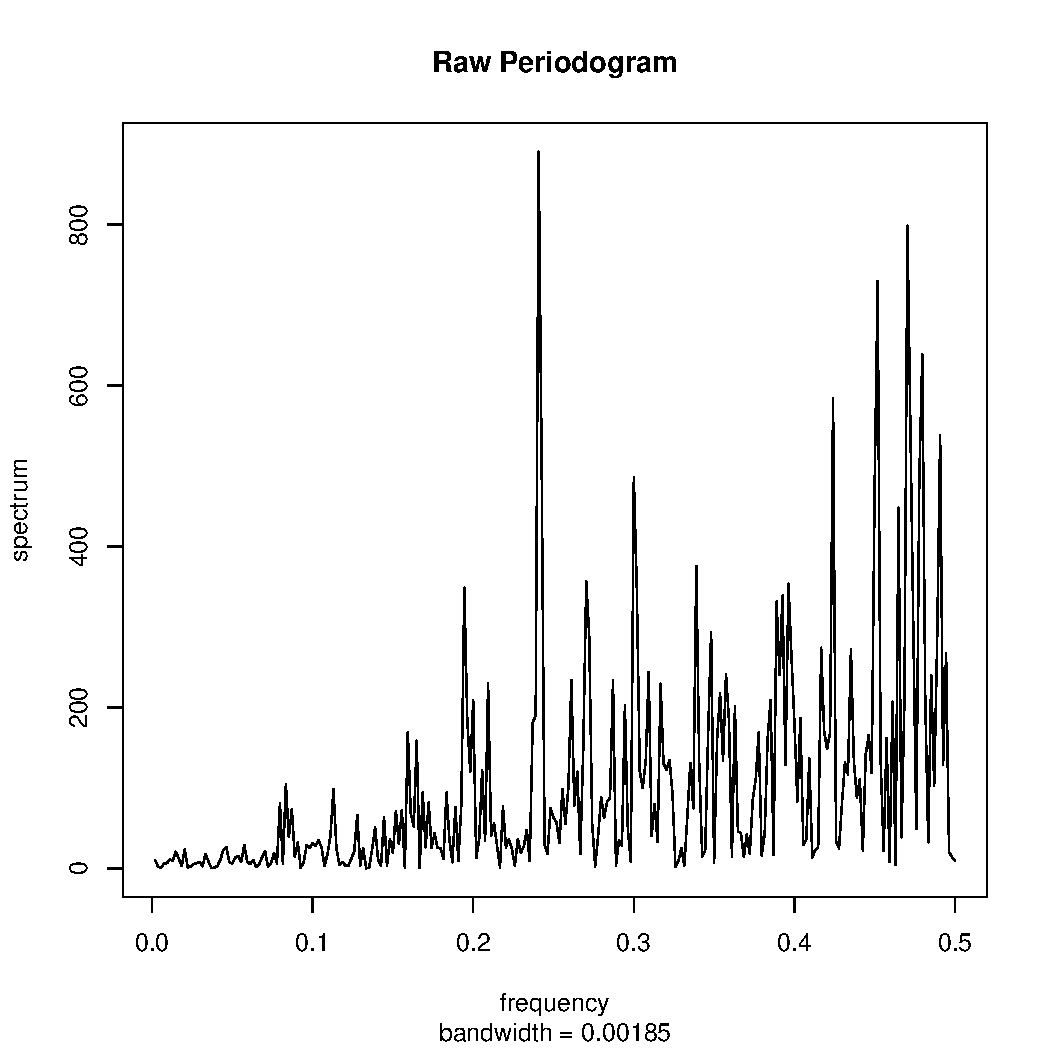
\includegraphics[width=0.45\linewidth]{../image/raw_periodogram.pdf}
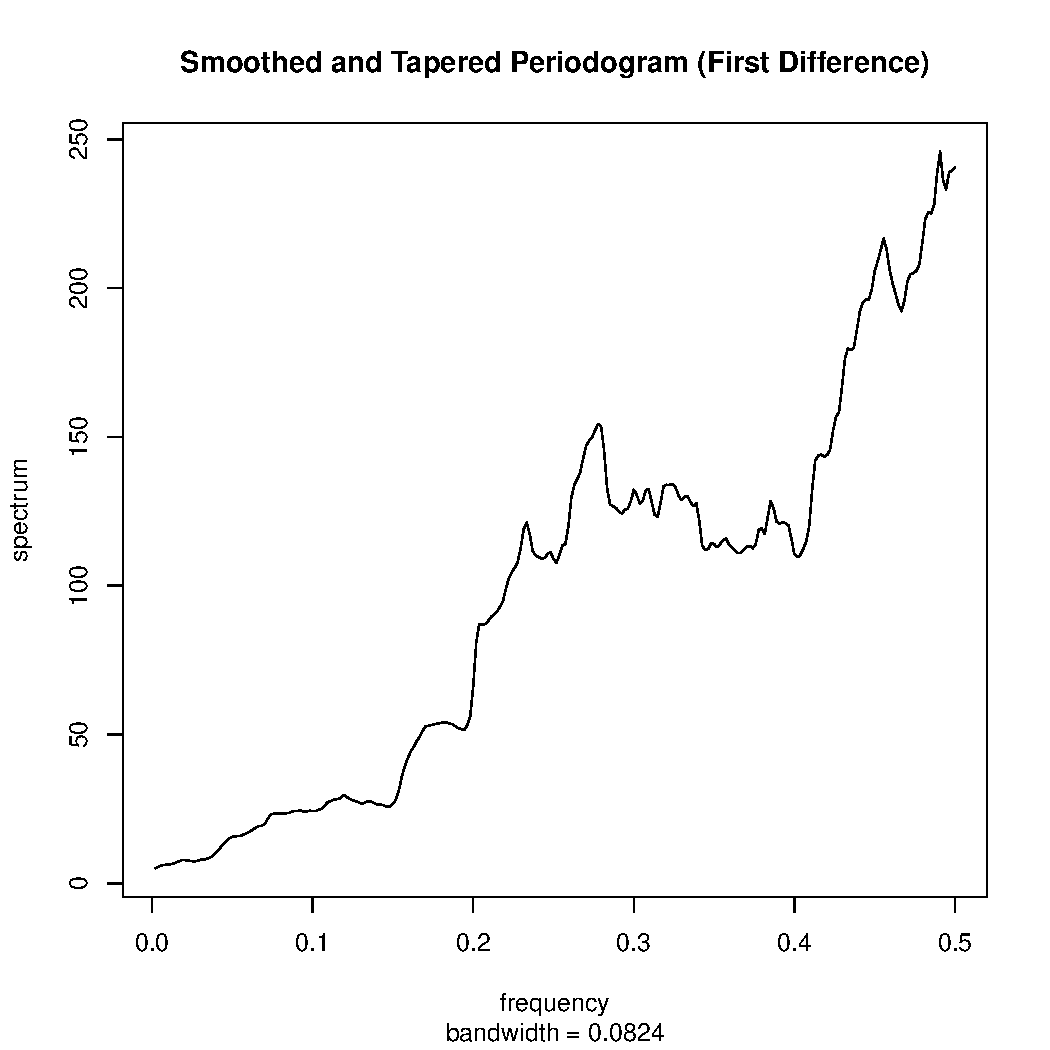
\includegraphics[width=0.45\linewidth]{../image/smooth_tapered_periodogram.pdf}
\caption{The Periodogram (left) and a Smoothed and Tapered Periodogram (right). Smoothed with a Daniell Kerenel with window??TODO?? size $m = \sqrt{n} \approx 22$ and tapered with ??cosine bell taper with? ?val? $0.1$}
\label{periodogram}
\end{figure}



\begin{figure}
\centering
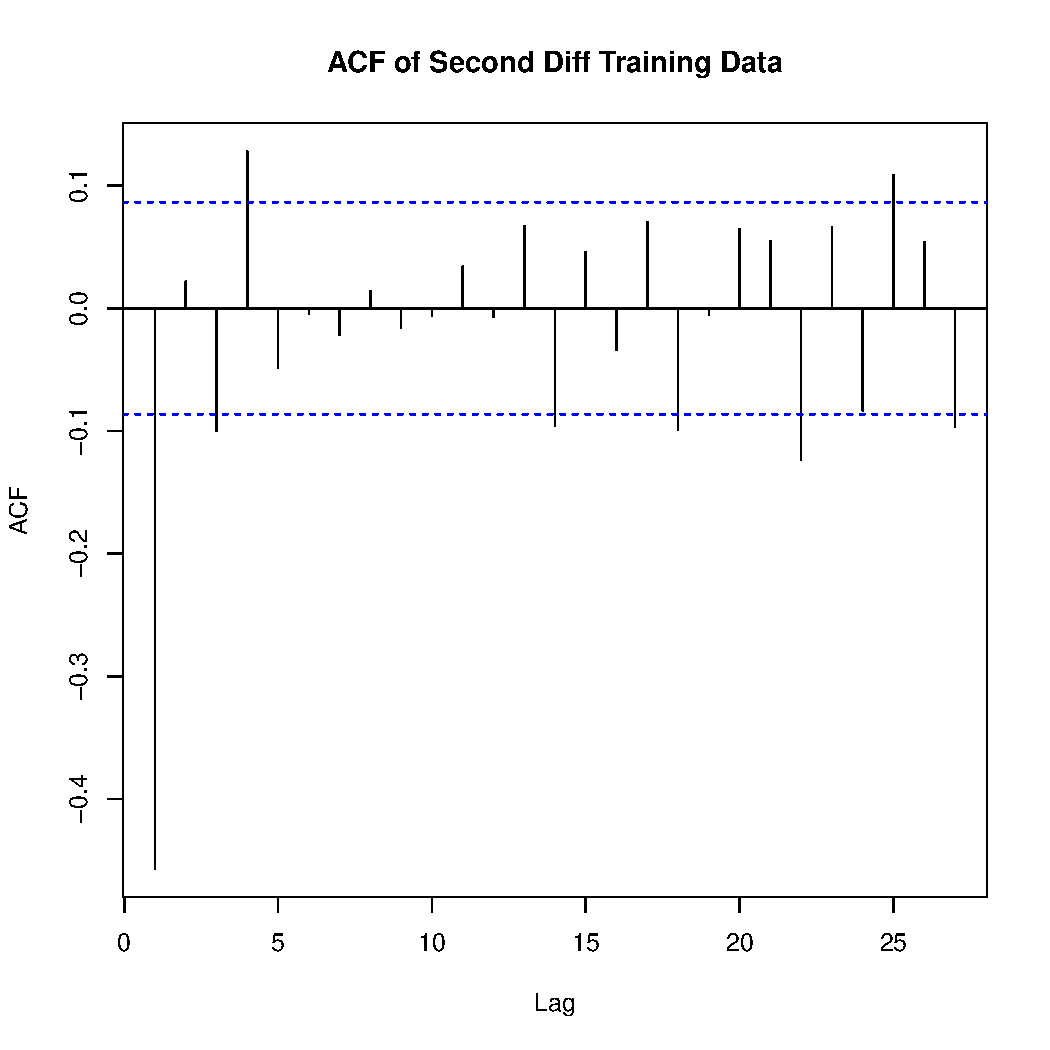
\includegraphics[width=0.45\linewidth]{../image/acf_second_diff.pdf}
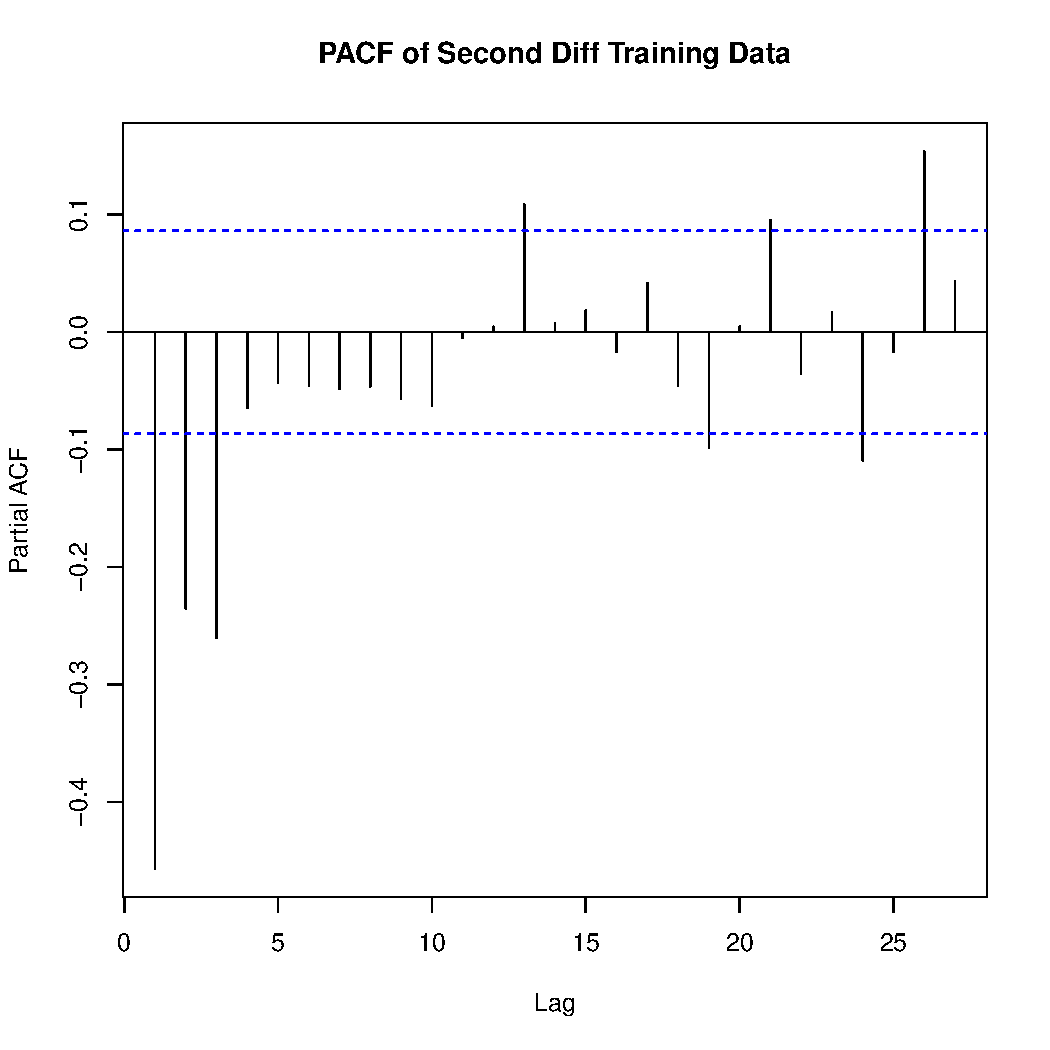
\includegraphics[width=0.45\linewidth]{../image/pacf_second_diff.pdf}
\caption{The ACF and PACF of the second diff time series}
\label{second_acf_pacf}
\end{figure}

\begin{figure}
\centering
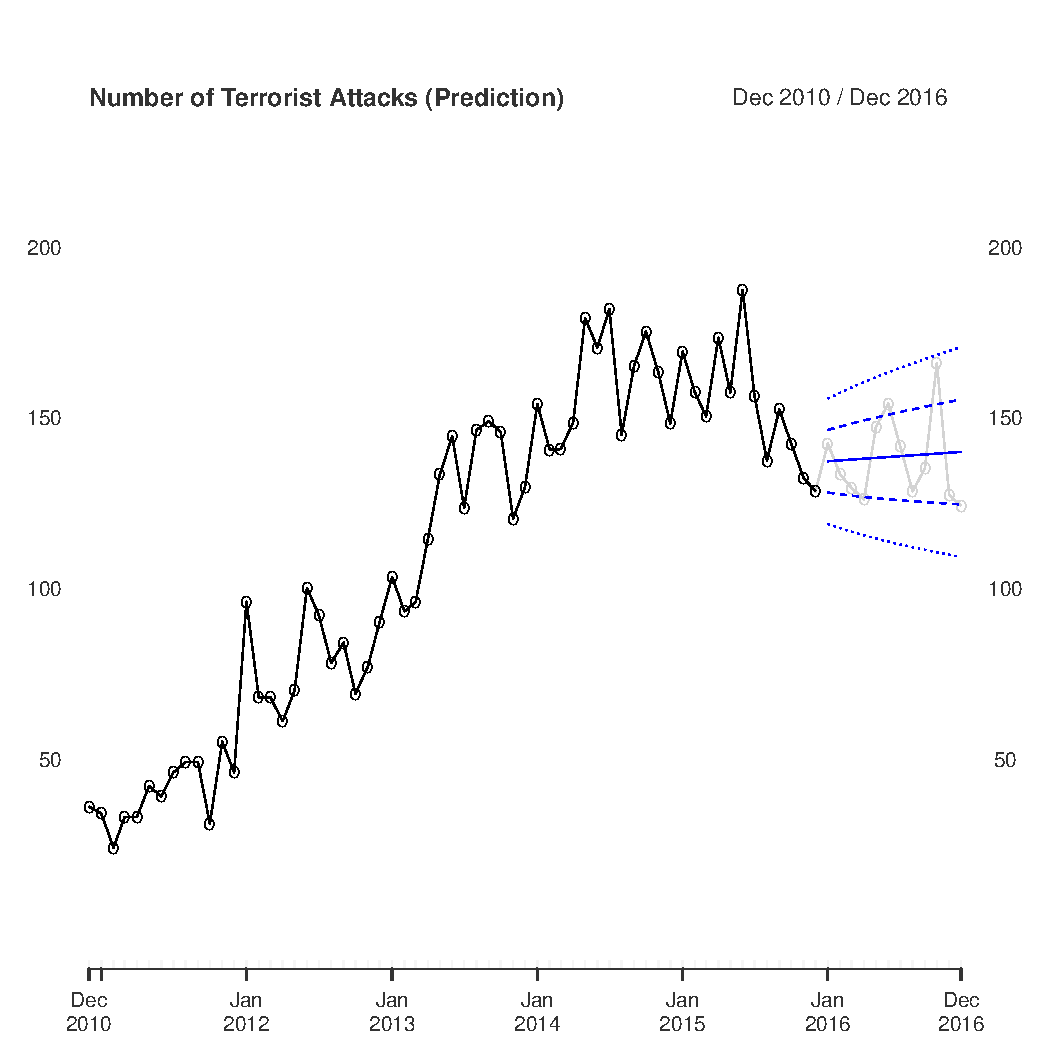
\includegraphics[width=0.75\linewidth]{../image/prediction_on_testing.pdf}
\caption{We use the model ---------- to generate a 12 month prediction denoted by the blue line. 1 sd and 2 sd error bars are the dotted lines. What actually occured is shown by the light gray.}
\label{prediction}
\end{figure}

\begin{figure}[t]
\centering
    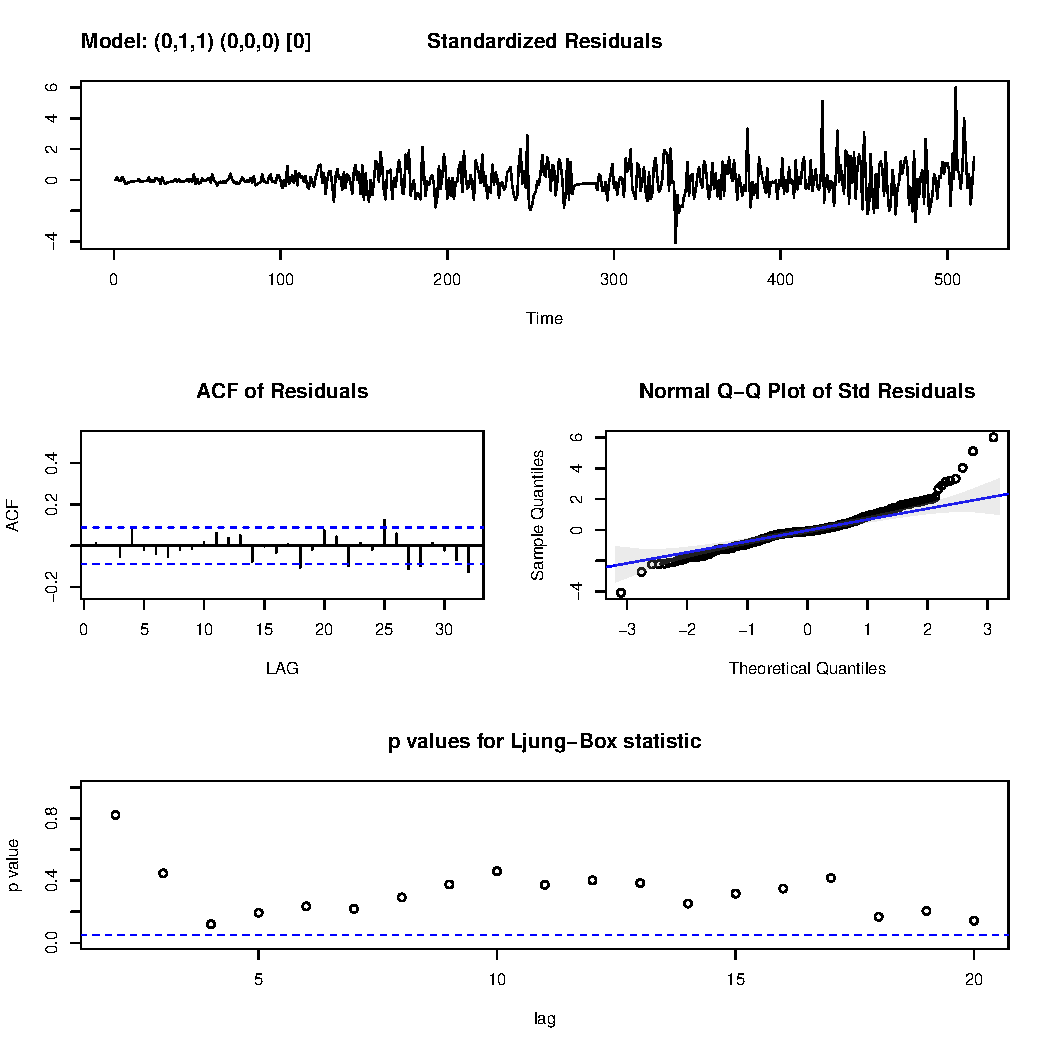
\includegraphics[width=0.75\textwidth]{../image/best_model.pdf}
\caption{This is the information from our best model.}
\label{outlier}
\end{figure}


\section{Data Analysis}
\section{Conclusion}

From the 
\begin{table}
\centering
\begin{tabular}{r || r | r| r| r}
$(p, d, q) \times(P, D, Q)_s$   & AIC   &AICc   &BIC    &MSE\\
\hline
$(0, 1, 1)$               & 5.248 &5.252  &4.265  &13212.18\\
$(0, 1, 1) \times (1, 0, 1)_4$   & 5.237 &5.241  &4.270  &13451.05\\ % Small p-values and passes ljung box p-values on seasonal ar1 and ma1; passes ljung box
$(0, 1, 1) \times (1, 1, 1)_4$   & 5.249 &5.254  &4.274  &13325.71\\
$(0, 1, 1) \times (1, 1, 2)_4$   & 5.242 &5.246  &4.275  &13728.1\\
\hline
$(1, 1, 2)$               & 5.256 & 5.260 &4.288  &13237.34\\
$(1, 1, 2) \times (1, 0, 1)_4$   & 5.243 &5.247  &4.292  &13785.23\\ %Large p-values on ma2, small 
$(1, 1, 2) \times (1, 1, 1)_4$   & 5.252 & 5.257 &4.294  &14144.5\\
$(1, 1, 2)\times (1, 1, 2)_4$   & 5.250 & 5.254 & 4.299 &13826.03
\end{tabular}
\caption{The metrics associated with different SARIMA models denoted by the left hand column.}
\end{table}

%For (terror4, 0, 1, 4, 1, 0, 1, 4) only ma1 coefficient was significant; it did pass ljung box.

\begin{table}
\centering
\begin{tabular}{r || r | r| r| r | r | r| r| r}%| r| r | r| r| r| r}
 AR/MA &0& 1& 2& 3& 4& 5& 6& 7\\%& 8& 9& 10& 11& 12& 13 \\
 \hline
 \hline
0&x&o&x&x&o&o&o&o\\%&o&o&o&o&o&x\\
1&x&x&o&x&o&o&o&o\\%&o&o&o&o&o&o\\
2&x&x&x&x&o&o&o&o\\%&o&o&o&o&o&o\\
3&x&x&x&x&o&o&o&o\\%&o&o&o&o&o&o\\
4&x&o&o&o&o&o&o&o\\%&o&o&o&o&o&o\\
5&x&x&o&o&o&o&o&o\\%&o&o&o&o&o&o\\
6&x&x&o&o&o&o&o&o\\%&o&o&o&o&o&o\\
7&x&x&o&o&o&o&o&o\\%&o&o&o&o&o&o
\end{tabular}
\begin{tabular}{r || r | r| r| r | r | r| r| r}%| r| r | r| r| r| r}
AR/MA&  0 &1& 2 &3& 4& 5& 6& 7\\%& 8& 9& 10& 11 &12 &13\\
\hline
\hline
0&x&x&x&x&o&o&o&o\\%&o&o&o&o&o&x\\
1&x&x&x&x&o&o&o&o\\%&o&o&o&o&o&o\\
2&x&x&x&x&o&o&o&o\\%&o&o&o&o&o&o\\
3&x&o&o&o&o&o&o&o\\%&o&o&o&o&o&o\\
4&x&x&o&o&o&o&o&o\\%&o&o&o&o&o&o\\
5&x&x&o&o&o&o&x&o\\%&o&o&o&o&o&o\\
6&x&x&x&o&o&o&o&o\\%&o&o&o&o&o&o\\
7&x&x&o&o&o&o&o&o\\%&o&o&o&o&o&o
\end{tabular}
\caption{The EACF table for once diffed (left) and twice diffed data (right). The "o" points represent values that are candidate models.}
\end{table}





\end{document} 

